\documentclass[12pt]{report}
\usepackage[utf8]{inputenc}
\usepackage{graphicx}
\usepackage{amsmath}
\usepackage{url} 
\usepackage{caption}
\usepackage{subcaption}
\usepackage{float}
\usepackage[portuguese]{babel}

\title{Análise Comparativa de Formatos de Mídia: PNG, JPEG, SVG, MP3, AAC, FLAC}
\author{João Pedro Rodrigues Leite}
\date{\today}

\begin{document}
	
	\maketitle
	
	\section{Introdução}
	Os formatos de mídia digital, como imagens e áudio, desempenham um papel importante no armazenamento e transmissão de informações digitais. O crescente uso da internet e de dispositivos móveis exige que esses formatos sejam eficientes em termos de armazenamento, largura de banda e qualidade. Formatos como PNG, JPEG, SVG, MP3, AAC e FLAC foram desenvolvidos para atender a essas necessidades, cada um com características técnicas específicas.
	
	Este relatório realiza uma análise comparativa entre esses formatos mais utilizados, considerando suas características técnicas, vantagens e desvantagens. A escolha correta do formato pode impactar de forma significativa a qualidade da mídia, o tempo de carregamento e a experiência do usuário, e este relatório explora essas diferenças.

	
	\section{Formatos de Imagem} Imagens são um dos tipos de mídia mais comuns, usadas em aplicações como websites, fotografia digital e design gráfico. Os três formatos mais utilizados são PNG, JPEG e SVG, cada um com características distintas em termos de compressão e qualidade.
	
	Uma diferença importante é que PNG e JPEG são formatos baseados em bitmap, enquanto o SVG é um formato vetorial. Essa distinção afeta como cada formato lida com redimensionamento e a qualidade visual em diferentes tamanhos.

	\begin{figure}[H]
		\centering
		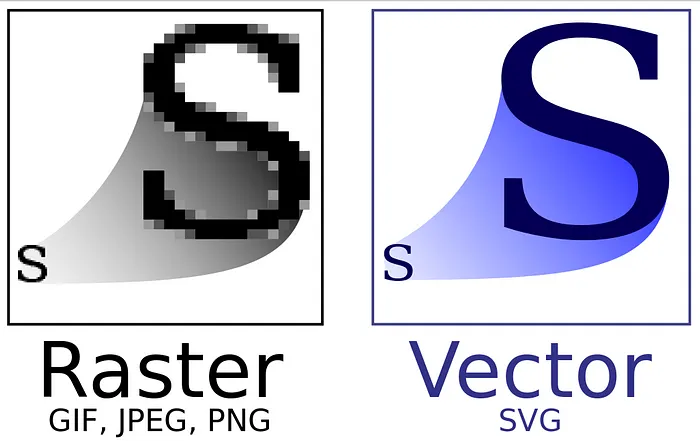
\includegraphics[width=0.5\linewidth]{figs/svgpng}
		\caption{Comparação de PNG, JPEG e GIF com SVG}
		\label{fig:svgpng}
		\caption*{Adaptado de: \cite{glasgow2024}}
	\end{figure}
	
	
	\subsection{PNG}
	O PNG (\textit{Portable Network Graphics}) é um formato sem perdas, mais adequado para imagens que exigem alta qualidade, como gráficos e logotipos. Sua maior vantagem é a capacidade de suportar transparência e compressão sem perda de dados (lossless). O uso de PNG é comum em design web e interfaces de usuário \cite{webnial2023}.
	
	\subsubsection{Vantagens}
	\begin{itemize}
		\item Compressão sem perdas.
		\item Suporte a transparência.
		\item Ideal para gráficos detalhados e imagens com texto.
	\end{itemize}
	
	\subsubsection{Desvantagens}
	\begin{itemize}
		\item Tamanho de arquivo maior em comparação ao JPEG.
		\item Não ideal para fotos devido à baixa eficiência na compressão de imagens complexas.
	\end{itemize}
	
	\subsection{JPEG}
	O JPEG (\textit{Joint Photographic Experts Group}) é um formato com compressão com perdas, amplamente utilizado em fotografias. Sua principal vantagem é a significativa redução de tamanho de arquivo, o que o torna ideal para aplicações que exigem o armazenamento de grandes quantidades de imagens \cite{techtudo2023}.
	
	\subsubsection{Vantagens}
	\begin{itemize}
		\item Compressão eficiente para fotos e imagens complexas.
		\item Tamanho de arquivo menor em comparação com o PNG.
		\item Amplamente compatível com plataformas digitais.
	\end{itemize}
	
	\subsubsection{Desvantagens}
	\begin{itemize}
		\item Compressão com perda, resultando em redução da qualidade.
		\item Não suporta transparência.
	\end{itemize}
	
	\subsection{SVG}
	O SVG (\textit{Scalable Vector Graphics}) é um formato de imagem vetorial baseado em XML, que permite a criação de gráficos que podem ser escalados para qualquer tamanho sem perda de qualidade. É amplamente utilizado para logotipos, ícones e gráficos interativos em websites \cite{w3c2023}.
	
	\subsubsection{Vantagens}
	\begin{itemize}
		\item Escalabilidade sem perda de qualidade.
		\item Suporte a gráficos interativos e animações.
		\item Arquivos geralmente menores para gráficos simples.
	\end{itemize}
	
	\subsubsection{Desvantagens}
	\begin{itemize}
		\item Pode se tornar complexo e grande para gráficos detalhados e muito elaborados.
		\item Não é ideal para imagens fotográficas ou altamente detalhadas.
	\end{itemize}
	
	\section{Formatos de Áudio}
	No contexto do áudio, o formato MP3 se tornou o padrão de fato para música e transmissões digitais, oferecendo uma boa compressão com qualidade satisfatória. Além do MP3, analisamos os formatos AAC e FLAC.
	
	\subsection{MP3}
	O MP3 (\textit{MPEG-1 Audio Layer III}) revolucionou o armazenamento e a distribuição de áudio ao introduzir uma forma de compressão com perda que reduz significativamente o tamanho dos arquivos de música sem uma degradação perceptível para a maioria dos ouvintes \cite{aero2024}.

	
	\subsubsection{Vantagens}
	\begin{itemize}
		\item Compressão eficiente com boa qualidade sonora.
		\item Pequenos tamanhos de arquivo, facilitando o armazenamento e a transmissão.
		\item Suporte universal em dispositivos e plataformas.
	\end{itemize}
	
	\subsubsection{Desvantagens}
	\begin{itemize}
		\item Perda de qualidade em compressões mais agressivas.
		\item Não ideal para áudio de alta fidelidade, como áudios profissionais.
	\end{itemize}
	
	\subsection{AAC}
	O AAC (\textit{Advanced Audio Coding}) é um formato de áudio com compressão com perdas, desenvolvido como uma evolução do MP3. Ele é projetado para oferecer melhor qualidade sonora a taxas de bits mais baixas, o que o torna ideal para aplicações de streaming e transmissão.
	
	\subsubsection{Vantagens}
	\begin{itemize}
		\item Melhor qualidade de áudio em comparações com MP3 a taxas de bits semelhantes.
		\item Suporte em uma ampla gama de dispositivos e plataformas.
		\item Menor tamanho de arquivo para a mesma qualidade sonora.
	\end{itemize}
	
	\subsubsection{Desvantagens}
	\begin{itemize}
		\item Compressão com perda, o que pode afetar a qualidade em compressões mais agressivas.
		\item Menos suporte universal em comparação com MP3.
	\end{itemize}
	
	\subsection{FLAC}
	O FLAC (\textit{Free Lossless Audio Codec}) é um formato de áudio com compressão sem perdas que preserva a qualidade original do áudio, ao mesmo tempo que reduz o tamanho do arquivo. É amplamente utilizado por entusiastas de áudio e profissionais que exigem qualidade máxima \cite{aero2024}.
	
	\subsubsection{Vantagens}
	\begin{itemize}
		\item Compressão sem perdas, preservando a qualidade original do áudio.
		\item Ideal para armazenamento de coleções de áudio em alta fidelidade.
		\item Suporte a metadados extensivos e tagueamento.
	\end{itemize}
	
	\subsubsection{Desvantagens}
	\begin{itemize}
		\item Tamanho de arquivo maior em comparação com formatos com perdas como MP3 e AAC.
		\item Menos suporte em dispositivos móveis e plataformas de streaming.
	\end{itemize}

	\section{Comparação entre os Formatos de Imagem}
	Cada formato de imagem discutido tem suas vantagens e desvantagens. Para imagens que exigem transparência ou alta qualidade, o PNG é preferido devido à sua compressão sem perdas e suporte a transparência. Por outro lado, o JPEG é ideal para fotografias onde o tamanho do arquivo é uma preocupação, oferecendo uma compressão eficiente para fotos e imagens complexas. Para gráficos escaláveis e interativos, o SVG é a melhor escolha, pois permite escalabilidade sem perda de qualidade e suporta animações e gráficos interativos.
	
	\section{Comparação entre os Formatos de Áudio}
	Já na comparação dos formatos de áudio, o MP3 continua sendo a escolha para a maioria dos usuários devido à sua compressão eficiente e suporte universal. No entanto, formatos como AAC oferecem melhor qualidade a taxas de bits semelhantes, tornando-os ideais para aplicações de streaming e transmissão. Para aqueles que buscam áudio de alta fidelidade, o FLAC é preferido, pois preserva a qualidade original do áudio com compressão sem perdas, apesar de ter um tamanho de arquivo maior em comparação com os formatos com perdas como MP3 e AAC.

	\section{Conclusão}
	A escolha do formato de mídia ideal depende das necessidades específicas de cada aplicação. No caso das imagens, o PNG é mais adequado para situações que exigem alta qualidade e transparência, enquanto o JPEG oferece uma boa compressão para fotografias. O SVG é a melhor opção para gráficos vetoriais escaláveis e interativos.
	
	Para áudio, o MP3 é amplamente utilizado devido à sua eficiência e compatibilidade, mas o AAC se destaca por oferecer melhor qualidade a taxas de bits equivalentes, tornando-o ideal para streaming. Já o FLAC é indicado para quem busca alta fidelidade, por preservar a qualidade original com compressão sem perdas.
	
	Compreender essas diferenças ajuda a equilibrar qualidade, tamanho de arquivo e compatibilidade, permitindo uma escolha mais estratégica de formato para cada tipo de conteúdo.

	
	\begin{thebibliography}{9}
		\bibitem{webnial2023}
		WEBNIAL. \textit{Formato de imagens: diferença entre JPEG e PNG}. Webnial, 2023. Disponível em: \url{https://webnial.pt/blog/formato-de-imagens-diferenca-entre-jpeg-e-png/}. Acesso em: 11 set. 2024.
		
		\bibitem{techtudo2023}
		TECHTUDO. \textit{Formatos de arquivos de imagem: entenda o que é JPG, GIF, PNG e mais}. TechTudo, 2023. Disponível em:\url{https://www.techtudo.com.br/noticias/2023/01/formatos-de-arquivos-de-imagem-entenda-o-que-e-jpg-gif-png-e-mais.ghtml}. Acesso em: 11 set. 2024.
		
		\bibitem{aero2024}
		AERO ENGENHARIA. \textit{O que é Algoritmo de Compressão de Imagem}. Aero Engenharia, 2024. Disponível em: \url{https://aeroengenharia.com/glossario/o-que-e-algoritmo-de-compressao-de-imagem/}. Acesso em: 11 set. 2024.
		
		\bibitem{w3c2023}
		WORLD WIDE WEB CONSORTIUM (W3C). \textit{Scalable Vector Graphics (SVG) Specification}. 2023. Disponível em: \url{https://www.w3.org/TR/SVG2/}.
		Acesso em: 11 set. 2024.
				
		\bibitem{glasgow2024}
		GLASGOW, G. \textit{Choosing Your Graphics Wisely: SVG vs PNG}. Medium, 2024. Disponível em: \url{https://medium.com/@g.glasgow91/choosing-your-graphics-wisely-svg-vs-png-9b4655c77c0b}. Acesso em: 11 set. 2024.
		
	\end{thebibliography}
	
\end{document}
